\subsection{\centering Oral Argument Participation -- Justices}
\begin{figure}[H]
\centering
\caption{Total Word Counts (By Justice - OT2023)}
\vspace{2.5mm}
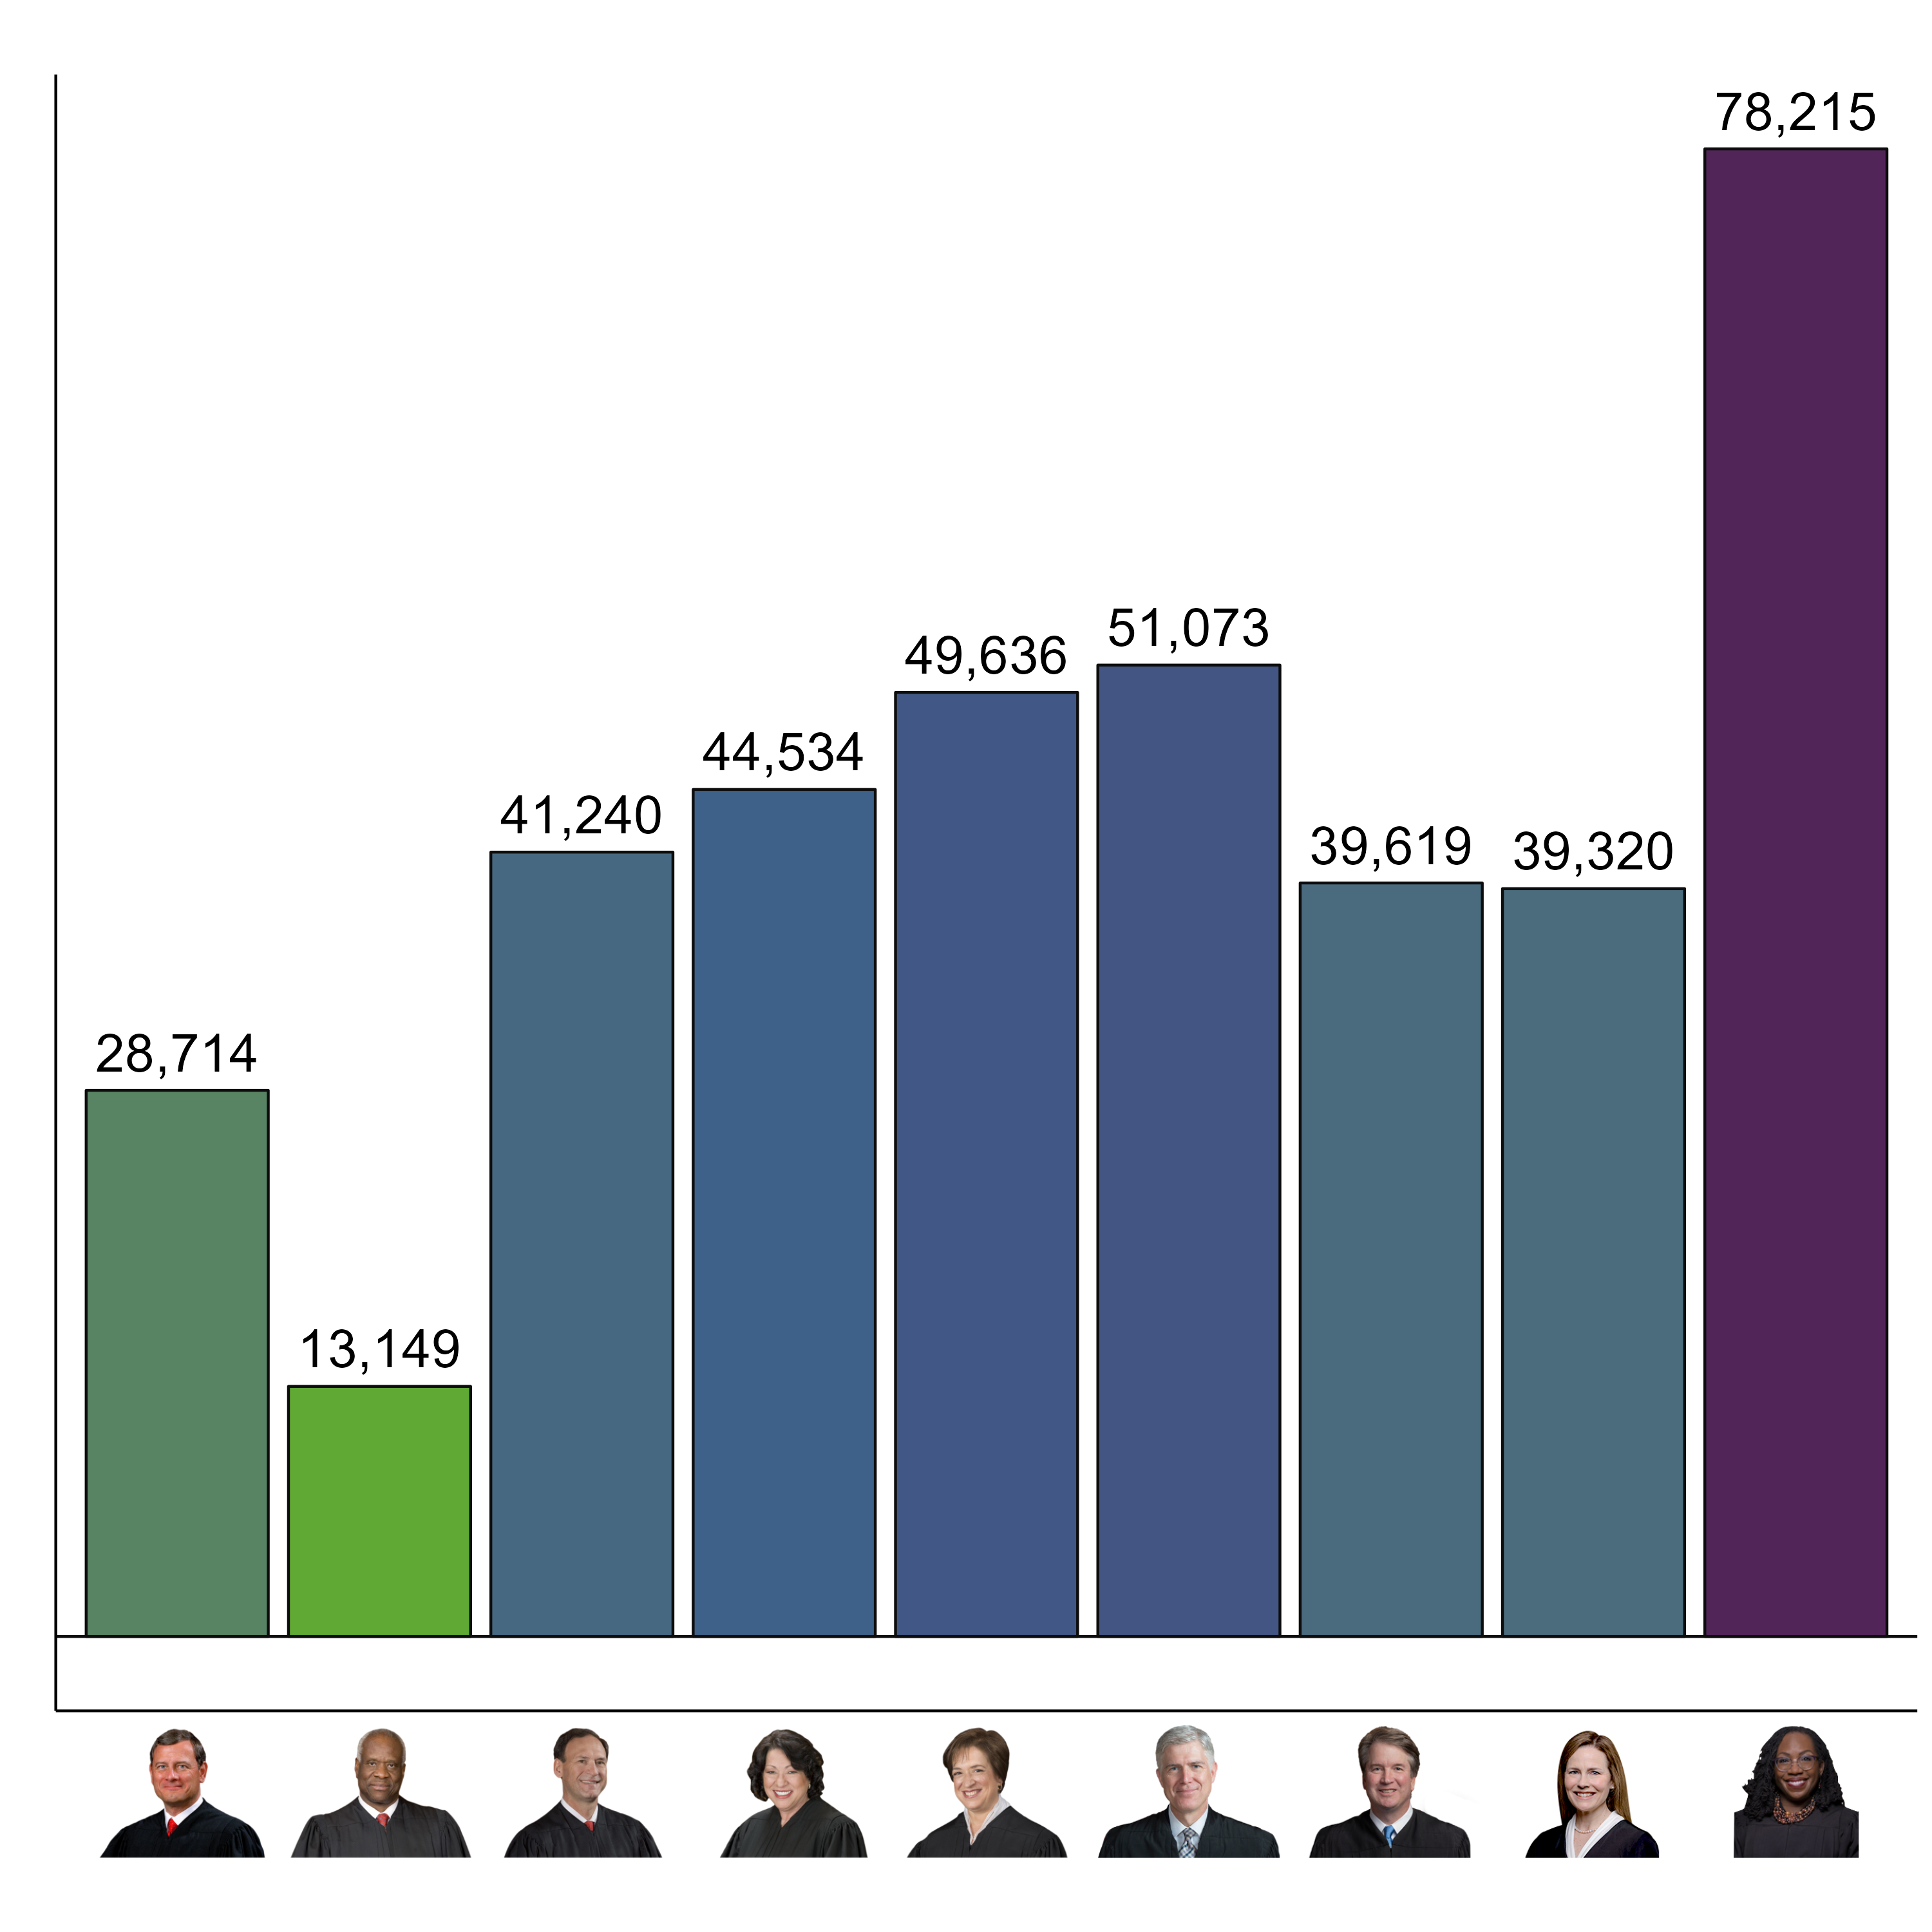
\includegraphics[width = 0.9\textwidth]{"Figures/statpack_figures/word_count_plot_OT23.png"} \\
\vspace{2mm}
\footnotesize{Data Source: Compiled from Oyez}
\end{figure}

\begin{landscape}
\subsection{\centering Oral Argument -- Word Counts (By Justice \& Argument)}
\begin{table}[H]
    \centering
    \renewcommand{\arraystretch}{1.5} % Add space between rows
    \caption{October Sitting (Word Counts)}
    \vspace{2mm}
    \csvreader[
        tabular= {L{0.3\textwidth}ccccccccc}, % Left-align the first column, Center-align rows 2 to 10
        table head = {
            \toprule
            \multicolumn{1}{c}{} &
            \multirow{3}{*}{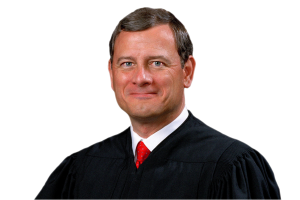
\includegraphics[width=1.5cm]{"Figures/justice_images/Roberts.png"}} &
            \multirow{3}{*}{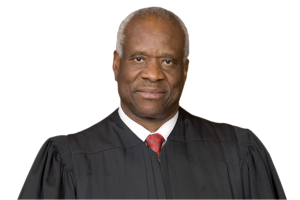
\includegraphics[width=1.5cm]{"Figures/justice_images/Thomas.png"}} &
            \multirow{3}{*}{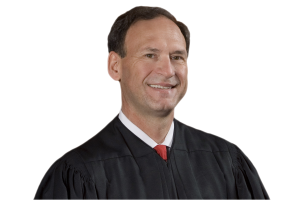
\includegraphics[width=1.5cm]{"Figures/justice_images/Alito.png"}} &
            \multirow{3}{*}{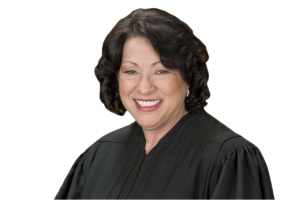
\includegraphics[width=1.5cm]{"Figures/justice_images/Sotomayor.png"}} &
            \multirow{3}{*}{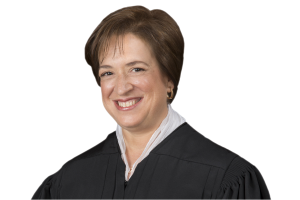
\includegraphics[width=1.5cm]{"Figures/justice_images/Kagan.png"}} &
            \multirow{3}{*}{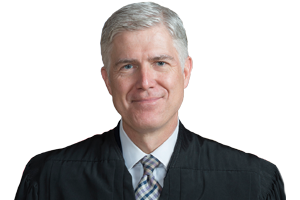
\includegraphics[width=1.5cm]{"Figures/justice_images/Gorsuch.png"}} &
            \multirow{3}{*}{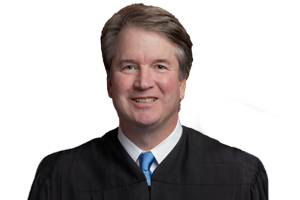
\includegraphics[width=1.5cm]{"Figures/justice_images/Kavanaugh.png"}} &
            \multirow{3}{*}{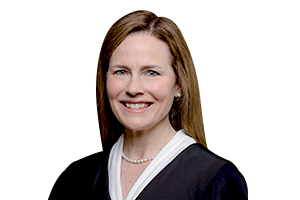
\includegraphics[width=1.5cm]{"Figures/justice_images/Barrett.png"}} &
            \multirow{3}{*}{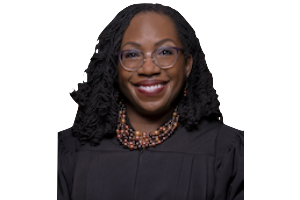
\includegraphics[width=1.5cm]{"Figures/justice_images/Jackson.png"}} \\
            & & & & & & & & & \\
            & \footnotesize{Roberts} & \footnotesize{Thomas} & \footnotesize{Alito} & \footnotesize{Sotomayor} & \footnotesize{Kagan} & \footnotesize{Gorsuch} & \footnotesize{Kavanaugh} & \footnotesize{Barrett} & \footnotesize{Jackson} \\
            \cmidrule{2-10}
        },
        table foot=\bottomrule \multicolumn{10}{l}{\footnotesize Data Source: Compiled from Oyez}\\ \bottomrule  % Specify the footer rule
    ]{"Tables/oral_argument_speaking/oral_argument_participation_October.csv"}{}%
    {\footnotesize \csvcoli & \multirow{1}{*}{\centering\csvcolii} & \multirow{1}{*}{\centering\csvcoliii} & \multirow{1}{*}{\centering\csvcoliv} & \multirow{1}{*}{\centering\csvcolv} & \multirow{1}{*}{\centering\csvcolvi} & \multirow{1}{*}{\centering\csvcolvii} & \multirow{1}{*}{\centering\csvcolviii} & \multirow{1}{*}{\centering\csvcolix} & \multirow{1}{*}{\centering\csvcolx}} % Specify all columns to include
    \label{tab:yourlabel}
\end{table}

\begin{table}[H]
    \centering
    \renewcommand{\arraystretch}{1.5} % Add space between rows
    \caption{November Sitting (Word Counts)}
    \vspace{2mm}
    \csvreader[
        tabular= {L{0.3\textwidth}ccccccccc}, % Left-align the first column, Center-align rows 2 to 10
        table head = {
            \toprule
            \multicolumn{1}{c}{} &
            \multirow{3}{*}{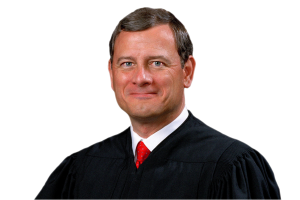
\includegraphics[width=1.5cm]{"Figures/justice_images/Roberts.png"}} &
            \multirow{3}{*}{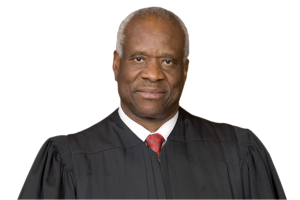
\includegraphics[width=1.5cm]{"Figures/justice_images/Thomas.png"}} &
            \multirow{3}{*}{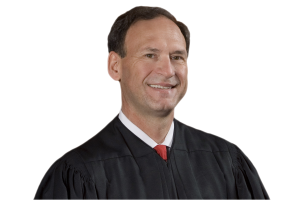
\includegraphics[width=1.5cm]{"Figures/justice_images/Alito.png"}} &
            \multirow{3}{*}{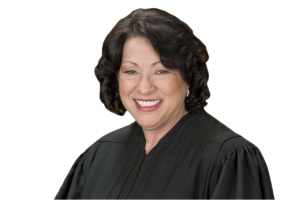
\includegraphics[width=1.5cm]{"Figures/justice_images/Sotomayor.png"}} &
            \multirow{3}{*}{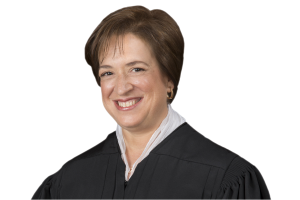
\includegraphics[width=1.5cm]{"Figures/justice_images/Kagan.png"}} &
            \multirow{3}{*}{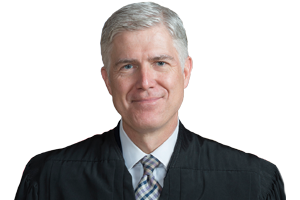
\includegraphics[width=1.5cm]{"Figures/justice_images/Gorsuch.png"}} &
            \multirow{3}{*}{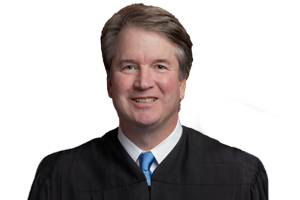
\includegraphics[width=1.5cm]{"Figures/justice_images/Kavanaugh.png"}} &
            \multirow{3}{*}{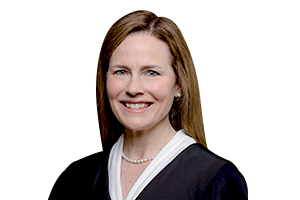
\includegraphics[width=1.5cm]{"Figures/justice_images/Barrett.png"}} &
            \multirow{3}{*}{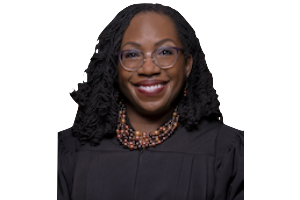
\includegraphics[width=1.5cm]{"Figures/justice_images/Jackson.png"}} \\
            & & & & & & & & & \\
            & \footnotesize{Roberts} & \footnotesize{Thomas} & \footnotesize{Alito} & \footnotesize{Sotomayor} & \footnotesize{Kagan} & \footnotesize{Gorsuch} & \footnotesize{Kavanaugh} & \footnotesize{Barrett} & \footnotesize{Jackson} \\
            \cmidrule{2-10}
        },
        table foot=\bottomrule \multicolumn{10}{l}{\footnotesize Data Source: Compiled from Oyez}\\ \bottomrule  % Specify the footer rule
    ]{"Tables/oral_argument_speaking/oral_argument_participation_November.csv"}{}%
    {\footnotesize \csvcoli & \multirow{1}{*}{\centering\csvcolii} & \multirow{1}{*}{\centering\csvcoliii} & \multirow{1}{*}{\centering\csvcoliv} & \multirow{1}{*}{\centering\csvcolv} & \multirow{1}{*}{\centering\csvcolvi} & \multirow{1}{*}{\centering\csvcolvii} & \multirow{1}{*}{\centering\csvcolviii} & \multirow{1}{*}{\centering\csvcolix} & \multirow{1}{*}{\centering\csvcolx}} % Specify all columns to include
    \label{tab:yourlabel}
\end{table}


\begin{table}[H]
    \centering
    \renewcommand{\arraystretch}{1.5} % Add space between rows
    \caption{December Sitting (Word Counts)}
    \vspace{2mm}
    \csvreader[
        tabular= {L{0.3\textwidth}ccccccccc}, % Left-align the first column, Center-align rows 2 to 10
        table head = {
            \toprule
            \multicolumn{1}{c}{} &
            \multirow{3}{*}{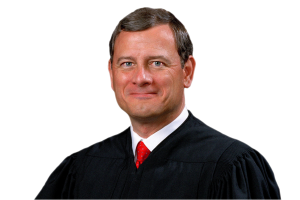
\includegraphics[width=1.5cm]{"Figures/justice_images/Roberts.png"}} &
            \multirow{3}{*}{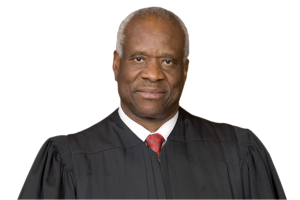
\includegraphics[width=1.5cm]{"Figures/justice_images/Thomas.png"}} &
            \multirow{3}{*}{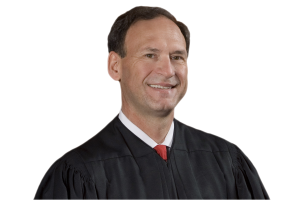
\includegraphics[width=1.5cm]{"Figures/justice_images/Alito.png"}} &
            \multirow{3}{*}{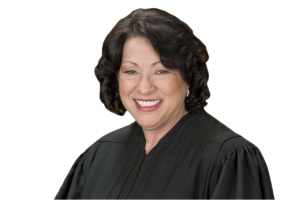
\includegraphics[width=1.5cm]{"Figures/justice_images/Sotomayor.png"}} &
            \multirow{3}{*}{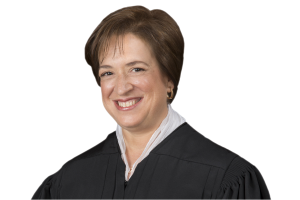
\includegraphics[width=1.5cm]{"Figures/justice_images/Kagan.png"}} &
            \multirow{3}{*}{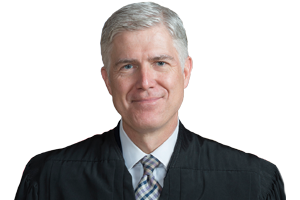
\includegraphics[width=1.5cm]{"Figures/justice_images/Gorsuch.png"}} &
            \multirow{3}{*}{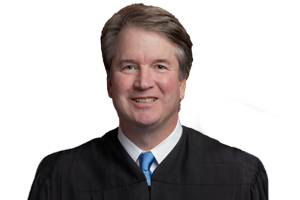
\includegraphics[width=1.5cm]{"Figures/justice_images/Kavanaugh.png"}} &
            \multirow{3}{*}{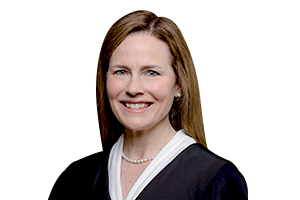
\includegraphics[width=1.5cm]{"Figures/justice_images/Barrett.png"}} &
            \multirow{3}{*}{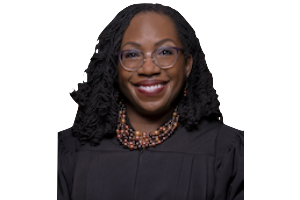
\includegraphics[width=1.5cm]{"Figures/justice_images/Jackson.png"}} \\
            & & & & & & & & & \\
            & \footnotesize{Roberts} & \footnotesize{Thomas} & \footnotesize{Alito} & \footnotesize{Sotomayor} & \footnotesize{Kagan} & \footnotesize{Gorsuch} & \footnotesize{Kavanaugh} & \footnotesize{Barrett} & \footnotesize{Jackson} \\
            \cmidrule{2-10}
        },
        table foot=\bottomrule \multicolumn{10}{l}{\footnotesize Data Source: Compiled from Oyez}\\ \bottomrule  % Specify the footer rule
    ]{"Tables/oral_argument_speaking/oral_argument_participation_December.csv"}{}%
    {\footnotesize \csvcoli & \multirow{1}{*}{\centering\csvcolii} & \multirow{1}{*}{\centering\csvcoliii} & \multirow{1}{*}{\centering\csvcoliv} & \multirow{1}{*}{\centering\csvcolv} & \multirow{1}{*}{\centering\csvcolvi} & \multirow{1}{*}{\centering\csvcolvii} & \multirow{1}{*}{\centering\csvcolviii} & \multirow{1}{*}{\centering\csvcolix} & \multirow{1}{*}{\centering\csvcolx}} % Specify all columns to include
    \label{tab:yourlabel}
\end{table}

\begin{table}[H]
    \centering
    \renewcommand{\arraystretch}{1.5} % Add space between rows
    \caption{January Sitting (Word Counts)}
    \vspace{2mm}
    \csvreader[
        tabular= {L{0.3\textwidth}ccccccccc}, % Left-align the first column, Center-align rows 2 to 10
       table head = {
            \toprule
            \multicolumn{1}{c}{} &
            \multirow{3}{*}{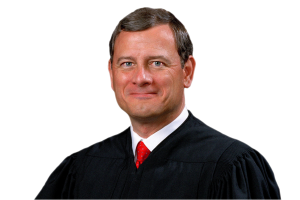
\includegraphics[width=1.5cm]{"Figures/justice_images/Roberts.png"}} &
            \multirow{3}{*}{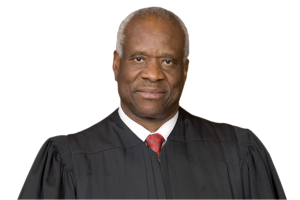
\includegraphics[width=1.5cm]{"Figures/justice_images/Thomas.png"}} &
            \multirow{3}{*}{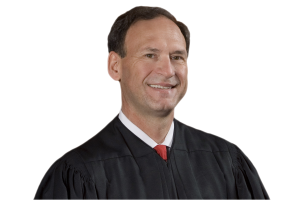
\includegraphics[width=1.5cm]{"Figures/justice_images/Alito.png"}} &
            \multirow{3}{*}{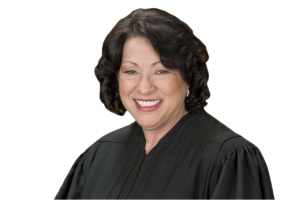
\includegraphics[width=1.5cm]{"Figures/justice_images/Sotomayor.png"}} &
            \multirow{3}{*}{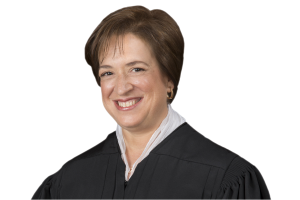
\includegraphics[width=1.5cm]{"Figures/justice_images/Kagan.png"}} &
            \multirow{3}{*}{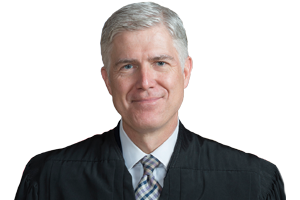
\includegraphics[width=1.5cm]{"Figures/justice_images/Gorsuch.png"}} &
            \multirow{3}{*}{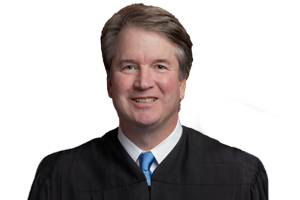
\includegraphics[width=1.5cm]{"Figures/justice_images/Kavanaugh.png"}} &
            \multirow{3}{*}{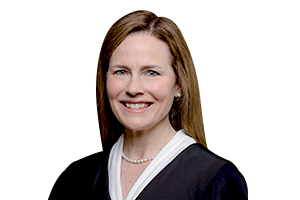
\includegraphics[width=1.5cm]{"Figures/justice_images/Barrett.png"}} &
            \multirow{3}{*}{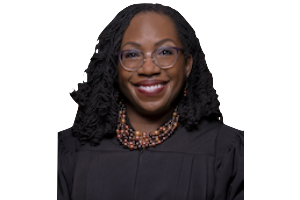
\includegraphics[width=1.5cm]{"Figures/justice_images/Jackson.png"}} \\
            & & & & & & & & & \\
            & \footnotesize{Roberts} & \footnotesize{Thomas} & \footnotesize{Alito} & \footnotesize{Sotomayor} & \footnotesize{Kagan} & \footnotesize{Gorsuch} & \footnotesize{Kavanaugh} & \footnotesize{Barrett} & \footnotesize{Jackson} \\
            \cmidrule{2-10}
        },
        table foot=\bottomrule \multicolumn{10}{l}{\footnotesize Data Source: Compiled from Oyez}\\ \bottomrule  % Specify the footer rule
    ]{"Tables/oral_argument_speaking/oral_argument_participation_January.csv"}{}%
    {\footnotesize \csvcoli & \multirow{1}{*}{\centering\csvcolii} & \multirow{1}{*}{\centering\csvcoliii} & \multirow{1}{*}{\centering\csvcoliv} & \multirow{1}{*}{\centering\csvcolv} & \multirow{1}{*}{\centering\csvcolvi} & \multirow{1}{*}{\centering\csvcolvii} & \multirow{1}{*}{\centering\csvcolviii} & \multirow{1}{*}{\centering\csvcolix} & \multirow{1}{*}{\centering\csvcolx}} % Specify all columns to include
    \label{tab:yourlabel}
\end{table}

\begin{table}[H]
    \centering
    \renewcommand{\arraystretch}{1.5} % Add space between rows
    \caption{February Sitting (Word Counts)}
    \vspace{2mm}
    \csvreader[
        tabular= {L{0.3\textwidth}ccccccccc}, % Left-align the first column, Center-align rows 2 to 10
       table head = {
            \toprule
            \multicolumn{1}{c}{} &
            \multirow{3}{*}{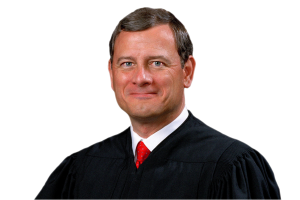
\includegraphics[width=1.5cm]{"Figures/justice_images/Roberts.png"}} &
            \multirow{3}{*}{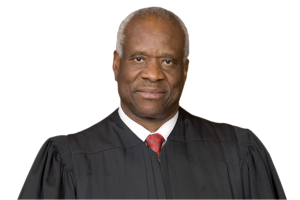
\includegraphics[width=1.5cm]{"Figures/justice_images/Thomas.png"}} &
            \multirow{3}{*}{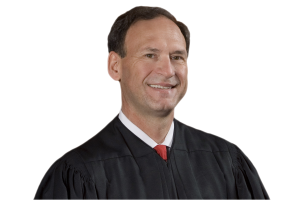
\includegraphics[width=1.5cm]{"Figures/justice_images/Alito.png"}} &
            \multirow{3}{*}{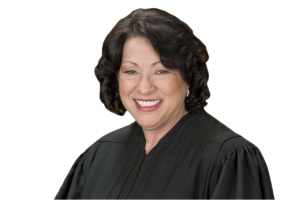
\includegraphics[width=1.5cm]{"Figures/justice_images/Sotomayor.png"}} &
            \multirow{3}{*}{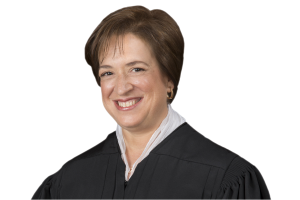
\includegraphics[width=1.5cm]{"Figures/justice_images/Kagan.png"}} &
            \multirow{3}{*}{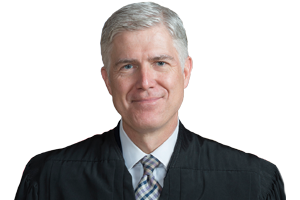
\includegraphics[width=1.5cm]{"Figures/justice_images/Gorsuch.png"}} &
            \multirow{3}{*}{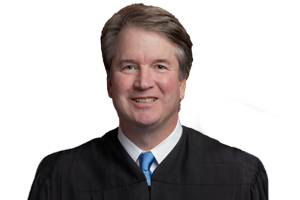
\includegraphics[width=1.5cm]{"Figures/justice_images/Kavanaugh.png"}} &
            \multirow{3}{*}{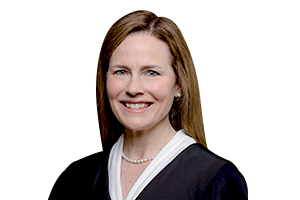
\includegraphics[width=1.5cm]{"Figures/justice_images/Barrett.png"}} &
            \multirow{3}{*}{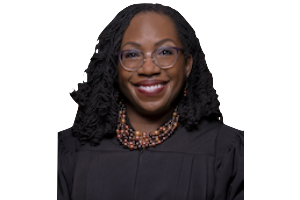
\includegraphics[width=1.5cm]{"Figures/justice_images/Jackson.png"}} \\
            & & & & & & & & & \\
            & \footnotesize{Roberts} & \footnotesize{Thomas} & \footnotesize{Alito} & \footnotesize{Sotomayor} & \footnotesize{Kagan} & \footnotesize{Gorsuch} & \footnotesize{Kavanaugh} & \footnotesize{Barrett} & \footnotesize{Jackson} \\
            \cmidrule{2-10}
        },
        table foot=\bottomrule \multicolumn{10}{l}{\footnotesize Data Source: Compiled from Oyez}\\ \bottomrule  % Specify the footer rule
    ]{"Tables/oral_argument_speaking/oral_argument_participation_February.csv"}{}%
    {\footnotesize \csvcoli & \multirow{1}{*}{\centering\csvcolii} & \multirow{1}{*}{\centering\csvcoliii} & \multirow{1}{*}{\centering\csvcoliv} & \multirow{1}{*}{\centering\csvcolv} & \multirow{1}{*}{\centering\csvcolvi} & \multirow{1}{*}{\centering\csvcolvii} & \multirow{1}{*}{\centering\csvcolviii} & \multirow{1}{*}{\centering\csvcolix} & \multirow{1}{*}{\centering\csvcolx}} % Specify all columns to include
    \label{tab:yourlabel}
\end{table}

\begin{table}[H]
    \centering
    \renewcommand{\arraystretch}{1.5} % Add space between rows
    \caption{March Sitting (Word Counts)}
    \vspace{2mm}
    \csvreader[
        tabular= {L{0.3\textwidth}ccccccccc}, % Left-align the first column, Center-align rows 2 to 10
        table head = {
            \toprule
            \multicolumn{1}{c}{} &
            \multirow{3}{*}{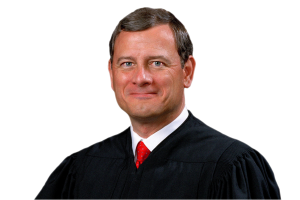
\includegraphics[width=1.5cm]{"Figures/justice_images/Roberts.png"}} &
            \multirow{3}{*}{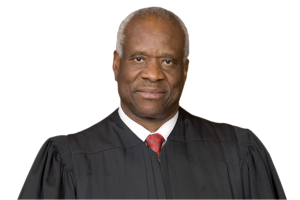
\includegraphics[width=1.5cm]{"Figures/justice_images/Thomas.png"}} &
            \multirow{3}{*}{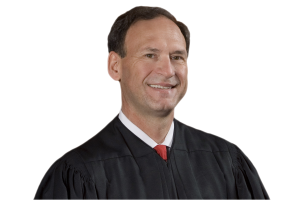
\includegraphics[width=1.5cm]{"Figures/justice_images/Alito.png"}} &
            \multirow{3}{*}{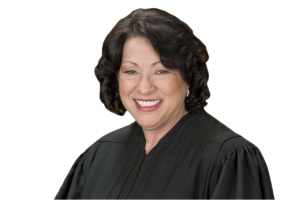
\includegraphics[width=1.5cm]{"Figures/justice_images/Sotomayor.png"}} &
            \multirow{3}{*}{\includegraphics[width=1.5cm]{"Figures/justice_images/Kagan.png"}} &
            \multirow{3}{*}{\includegraphics[width=1.5cm]{"Figures/justice_images/Gorsuch.png"}} &
            \multirow{3}{*}{\includegraphics[width=1.5cm]{"Figures/justice_images/Kavanaugh.png"}} &
            \multirow{3}{*}{\includegraphics[width=1.5cm]{"Figures/justice_images/Barrett.png"}} &
            \multirow{3}{*}{\includegraphics[width=1.5cm]{"Figures/justice_images/Jackson.png"}} \\
            & & & & & & & & & \\
            & \footnotesize{Roberts} & \footnotesize{Thomas} & \footnotesize{Alito} & \footnotesize{Sotomayor} & \footnotesize{Kagan} & \footnotesize{Gorsuch} & \footnotesize{Kavanaugh} & \footnotesize{Barrett} & \footnotesize{Jackson} \\
            \cmidrule{2-10}
        },
        table foot=\bottomrule \multicolumn{10}{l}{\footnotesize Data Source: Compiled from Oyez}\\ \bottomrule  % Specify the footer rule
    ]{"Tables/oral_argument_speaking/oral_argument_participation_March.csv"}{}%
    {\footnotesize \csvcoli & \multirow{1}{*}{\centering\csvcolii} & \multirow{1}{*}{\centering\csvcoliii} & \multirow{1}{*}{\centering\csvcoliv} & \multirow{1}{*}{\centering\csvcolv} & \multirow{1}{*}{\centering\csvcolvi} & \multirow{1}{*}{\centering\csvcolvii} & \multirow{1}{*}{\centering\csvcolviii} & \multirow{1}{*}{\centering\csvcolix} & \multirow{1}{*}{\centering\csvcolx}} % Specify all columns to include
    \label{tab:yourlabel}
\end{table}


\begin{table}[H]
    \centering
    \renewcommand{\arraystretch}{1.5} % Add space between rows
    \caption{April Sitting (Word Counts)}
    \vspace{2mm}
    \csvreader[
        tabular= {L{0.3\textwidth}ccccccccc}, % Left-align the first column, Center-align rows 2 to 10
        table head = {
            \toprule
            \multicolumn{1}{c}{} &
            \multirow{3}{*}{\includegraphics[width=1.5cm]{"Figures/justice_images/Roberts.png"}} &
            \multirow{3}{*}{\includegraphics[width=1.5cm]{"Figures/justice_images/Thomas.png"}} &
            \multirow{3}{*}{\includegraphics[width=1.5cm]{"Figures/justice_images/Alito.png"}} &
            \multirow{3}{*}{\includegraphics[width=1.5cm]{"Figures/justice_images/Sotomayor.png"}} &
            \multirow{3}{*}{\includegraphics[width=1.5cm]{"Figures/justice_images/Kagan.png"}} &
            \multirow{3}{*}{\includegraphics[width=1.5cm]{"Figures/justice_images/Gorsuch.png"}} &
            \multirow{3}{*}{\includegraphics[width=1.5cm]{"Figures/justice_images/Kavanaugh.png"}} &
            \multirow{3}{*}{\includegraphics[width=1.5cm]{"Figures/justice_images/Barrett.png"}} &
            \multirow{3}{*}{\includegraphics[width=1.5cm]{"Figures/justice_images/Jackson.png"}} \\
            & & & & & & & & & \\
            & \footnotesize{Roberts} & \footnotesize{Thomas} & \footnotesize{Alito} & \footnotesize{Sotomayor} & \footnotesize{Kagan} & \footnotesize{Gorsuch} & \footnotesize{Kavanaugh} & \footnotesize{Barrett} & \footnotesize{Jackson} \\
            \cmidrule{2-10}
        },
        table foot=\bottomrule \multicolumn{10}{l}{\footnotesize Data Source: Compiled from Oyez}\\ \bottomrule  % Specify the footer rule
    ]{"Tables/oral_argument_speaking/oral_argument_participation_April.csv"}{}%
    {\footnotesize \csvcoli & \multirow{1}{*}{\centering\csvcolii} & \multirow{1}{*}{\centering\csvcoliii} & \multirow{1}{*}{\centering\csvcoliv} & \multirow{1}{*}{\centering\csvcolv} & \multirow{1}{*}{\centering\csvcolvi} & \multirow{1}{*}{\centering\csvcolvii} & \multirow{1}{*}{\centering\csvcolviii} & \multirow{1}{*}{\centering\csvcolix} & \multirow{1}{*}{\centering\csvcolx}} % Specify all columns to include
    \label{tab:yourlabel}
\end{table}

\end{landscape}
